\documentclass[11p, titlepage, oneside, a4paper]{article}
% Packages
\usepackage{amsmath}
\usepackage{graphicx}
\usepackage{hyperref}
\usepackage[english,swedish]{babel}
\usepackage[
    backend=biber,
    style=authoryear-ibid,
    sorting=ynt
]{biblatex}
\usepackage[utf8]{inputenc}
\usepackage[T1]{fontenc}
\usepackage{tcolorbox}
\usepackage{booktabs}
%Källor
\addbibresource{mall.bib}
\graphicspath{ {./images/} }

% Ändra de rader som behöver ändras
\def\inst{Teknikprogrammet}
\def\typeofdoc{Laborationsrapport}
\def\course{Fysik 1 150p}
\def\pretitle{Laboration 2}
\def\title{Fjäder- och Friktionskraft}
\def\name{Henrik Forsberg}
\def\username{henrik.forsberg}
\def\email{\username{}@elev.ga.ntig.se}
\def\graders{Magnus Silverdal}

\begin{document}

\begin{titlepage}
		\thispagestyle{empty}
		\begin{large}
			\begin{tabular}{@{}p{\textwidth}@{}}
				\textbf{NTI gymnasiet \hfill \today} \\
				\textbf{\inst} \\
				\textbf{\typeofdoc} \\
			\end{tabular}
		\end{large}
		\vspace{10mm}
		\begin{center}
			\LARGE{\pretitle} \\
			\huge{\textbf{\course}}\\
			\vspace{10mm}
			\LARGE{\title} \\
			\vspace{15mm}
			\begin{large}
				\begin{tabular}{ll}
					\textbf{Namn} & \name \\
					\textbf{E-mail} & \texttt{\email} \\
				\end{tabular}
			\end{large}
			\vfill
            
\includegraphics[width=0.5\textwidth]{NTI Gymnasiet_Symbol_print_svart}
			\vfill
            \large{\textbf{Handledare}}\\
			\mbox{\large{\graders}}
		\end{center}
	\end{titlepage}

    \begin{otherlanguage}{english}
	\begin{abstract}
        This paper is about the relation between the spring force and it's length though measuring it with a differing amount of weight. It is also about the relation between the normal force and friction on a block on a tilting plane.
    \end{abstract}
    \end{otherlanguage}
    % Om arbetet är långt har det en innehållsförteckning, annars kan den utelämnas
	\pagenumbering{roman}
	\tableofcontents
	
	% och lägger in en sidbrytning
	\newpage

	\pagenumbering{arabic}
	
	% i Sverige har vi normalt inget indrag vid nytt stycke
	\setlength{\parindent}{0pt}
	% men däremot lite mellanrum
	\setlength{\parskip}{10pt}
	
	\section{Syfte och frågeställning}
        Syftet med laborationen är att analysera fjäderkonstaten för en fjärder samt undersöka hur olika vikt påverkar friktionen av en kloss.

	\section{Bakgrund och teori}
	    Fjäderkraft är kraften en fjäder utöver under en viss tidpunkt vilket räknas ut med följande formel m*g där g är gravitations konstanten (9,82) och m är massan av vikten i kg. Friktionskraften av klossen är m*g*sin(a) och normalkraften är m*g*sin(a). Mer utvecklad förklaring i figur \ref{fig:triangle}.

    \begin{figure}[!h]
        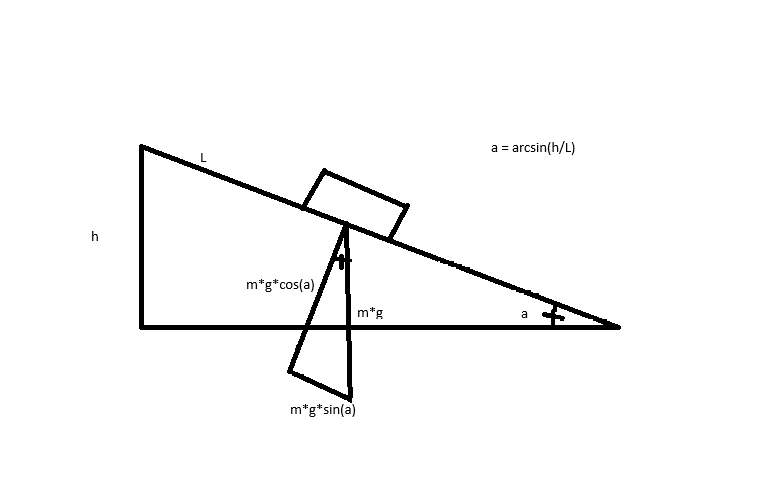
\includegraphics[width=0.8\textwidth]{friktionskraftexplain}
        \caption{Friktions- och normalkraft förklaring}
        \label{fig:triangle}
    \end{figure}


	\section{Metod och materiel}

        \subtitle{Fjäderkraft}

        \begin{enumerate}
            \item Fjäder
            \item Vikt (0,05kg)
            \item Ställning
            \item Linjal
        \end{enumerate}
        
        Fjädern monteras lodrätt i ställnignen. En vikt hängs i botten av fjädern och längden av fjädern mäts. En vikt läggs till och fjäderna mäts igen, detta upprepas till vi har 5 vikter, se figur \ref{fig:fjäderuppställning}.

        \begin{figure}[!h]
            \includegraphics[width=0.8\textwidth]{fjäderuppställning}
            \caption{Hur uppställningen såg ut}
            \label{fig:fjäderuppställning}
        \end{figure}

        \subtitle{Friktions- och normalkraft}

        \begin{enumerate}
            \item Kloss
            \item Vikt (0,05kg)
            \item Tejp
            \item Lutande plan
            \item Linjal
        \end{enumerate}
        
        En kloss lades på ett lutande plan som sedan lyftes fram till att klossen hade konstant acceleration. Sedan mättes höjden av den sidan som lyftes distans till bordet. Sedan gjordes testet igen fast med en till vikt fram till att den hade gjorts 5 gånger totalt \ref{fig:friktionsuppställning}.

        \begin{figure}[!h]
            \includegraphics[width=0.8\textwidth]{friktionsuppställning}
            \caption{Hur uppställningen såg ut}
            \label{fig:friktionsuppställning}
        \end{figure}

    \newpage
    \section{Analys och beräkning}
    Datan importeras i Excel och fjäderkraften beräknas med hjälp av funktionen av m*g. Friktions kraften räknas ut med m*g*sin(a) och normalkraften med m*g*cos(a) se figur \ref{fig:triangle}. Datan ger följande grafer:

    \begin{figure}[!h]
        \includegraphics[width=0.8\textwidth]{fjäderkraftgraf}
        \caption{Hur längden av fjädern förhåller sig till fjäderkraften}
        \label{fig:fjädergraf}
    \end{figure}

    \begin{figure}[!h]
        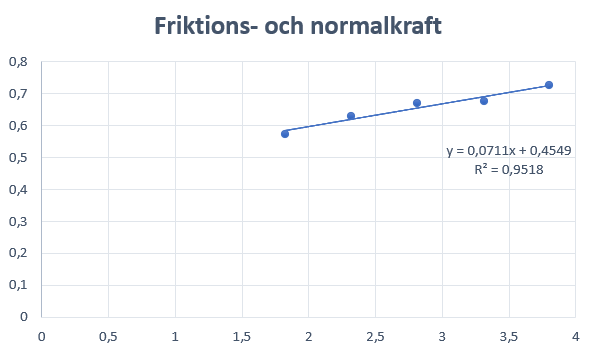
\includegraphics[width=0.8\textwidth]{Friktionsgraf}
        \caption{Hur normalkraften beror på friktionskraften}
        \label{fig:friktionsgraf}
    \end{figure}

    \section{Slutsats och resultat} 
        Resultatet av beräkningarna illustreras i graferna \ref{fig:fjädergraf} och \ref{fig:friktionsgraf}
    \section{Diskussion} 
    Eftersom att \(R^{2} = 1\) i fjäderkrafts diagrammet så lyder den vad som teoretikst skulle hända. Men den andra skulle också teoretiskt ha det. Anledningar till att den inte har det är mest troligt på grund av att hålla stilla medan någon mäter är ganska svårt så det kommer aldrig att bli helt rätt. Det är också svårt att se om accelerationen är 0 eller om den fortfarande accelererar lite.

    
    \printbibliography

\end{document}

